\section{Motivation}
\label{sec:motivation}
\subsection{Experiment Setup and Overview}
Our central hypothesis is that \textbf{decode-phase} throughput is largely determined by the memory access pattern of the KV cache rather than by compute. In particular, when all the requests in a batch share a common prefix, their attention operations traverse the same KV cache regions at roughly the same time. This aligned access pattern improves spatial and temporal locality in the GPU memory hierarchy, allowing the hardware to better utilize cache capacity and memory bandwidth. Conversely, when requests have heterogeneous prefixes, KV accesses become interleaved across disjoint regions of memory, disrupting locality and reducing effective bandwidth utilization. \textcolor{green}{Another goal which we wish to achieve through our experiments is to evaluate if we can reap locality gains without changing attention kernels.}

To validate this hypothesis, we design a series of controlled experiments that systematically vary (i) the amount of prefix sharing within a batch, (ii) the number of distinct prefix groups, and (iii) the batch size and decode length. Across these experiments, we measure decode throughput and memory behaviour to understand how prefix structure affects inference performance. Each experiment concludes with a takeaway summarizing the key insight.

All experiments use the LLama3-8B \cite{llama3modelcard} model.  Experiments are performed on an RTX6000 Ada Generation GPU \cite{nvidia_rtx6000_datasheet}, equipped with 48GB of GDDR6 memory and a 96MB L2 cache. We use the vLLM \cite{kwon2023efficient} inference engine with a default maximum batch size of 500 unless stated otherwise. We primarily focus on decode-phase throughput, measured in output tokens per second. To isolate decode behaviour, we perform a warm-up run such that all prefix KV caches are resident in GPU memory prior to measurement. This ensures that the per-token compute cost remains constant across experimental settings and that observed differences arise primarily from memory behaviour and batching effects. Later, we also compare end-to-end throughput, which includes the time taken to prefill the queries. For this model, a single 10k-token request generates approximately 1.4GB of KV cache data (across all layers, for both keys and values). Within each layer, KV tensors corresponding to consecutive tokens are stored contiguously in memory. We pick requests from the L-Eval \cite{an2023leval} dataset, and we prune the size of each request as required by the experiment. We use the FlashAttention~\cite{dao2022flashattentionfastmemoryefficientexact} backend throughout all the experiments.


\subsection{Locality and Sharing}
We begin by examining how \textit{prefix heterogeneity} within a batch affects decode throughput.  Prefix heterogeneity refers to the presence of requests with different input prefixes in the same batch.  When requests share the same prefix, they access the same KV cache regions during decode; when prefixes differ, the KV accesses correspond to different memory regions.

To quantify the impact of prefix heterogeneity, we design a controlled experiment with two large system prompts, $A$ and $B$, each of length $10{,}000$ tokens. We form a batch of $500$ requests, where each request consists of either prefix $A$ or $B$, followed by a unique suffix of length $20$ tokens (Figure~\ref{fig:two_fam_vis}). Each request then generates 50 decode tokens. Let $f \in [0,1]$ denote the fraction of requests using prefix $A$. When $f=0$ or $f=1$, the batch is homogeneous, and all $500$ requests share a single prefix. When $0 < f < 1$, two distinct prefix families coexist within the same batch. We do a warmup run before measuring the decode throughput, which ensures that the KV caches corresponding to both the prefix groups are already resident in the GPU memory, and the amount of compute involved is the same across all values of $f$.

Figure~\ref{fig:two_fam_tp} shows decode throughput as a function of $f$. Throughput is maximized when the batch is homogeneous ($f = 0$ or $f = 1$). However, introducing even a single request from the other prefix family causes a sharp degradation. Specifically, at $f = 0.002$ (one request out of $500$), throughput drops by nearly $2\times$. This demonstrates that decode throughput is extremely sensitive to even minimal prefix heterogeneity within a small batch.

\begin{figure}[H]
    \centering
    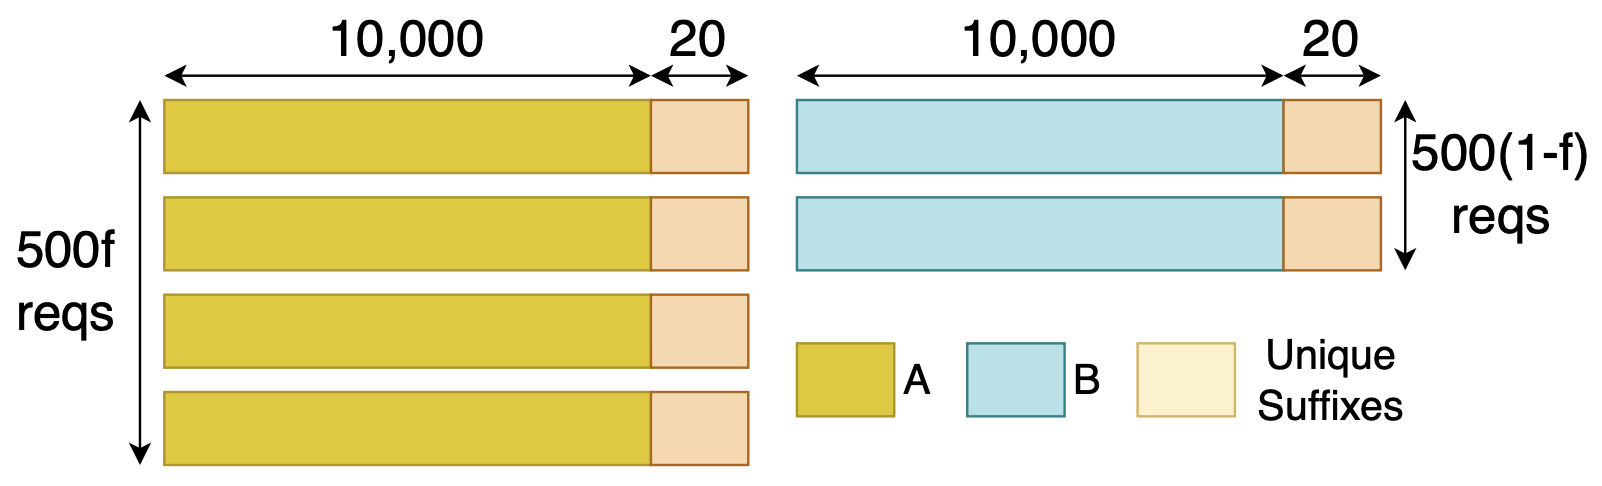
\includegraphics[width=\linewidth]{illustration_images/two_family_experiment.png}
    \caption{Visualization of Heterogeneous Batches}
    \label{fig:two_fam_vis}
\end{figure}
\textcolor{red}{Do we need to mark fractions such as $0.002$ or $0.01$ more clearly in this graph?}

To better understand this effect, we measure mean DRAM activity, defined as the fraction of cycles during which the DRAM pipe is active. As shown in Figure~\ref{fig:two_fam_mean_dram}, homogeneous batches exhibit over $50\%$ higher DRAM activity compared to mixed-prefix settings.

A $10$k-token prefix corresponds to over $1$GB of KV cache data (across all layers). Even with sharing across requests, the active KV working set during decode substantially exceeds the $96$MB L2 cache capacity of the GPU, particularly after accounting for model weights. Thus, decode is fundamentally memory-bound, and only a small portion of the KV cache can reside in L2 at any given time.

\textcolor{red}{present max bandwidth numbers here}

During each decode step, every request attends to its entire prefix. Because the prefix length (10k tokens) dominates both the decode length (50 tokens) and the query length, memory accesses are largely determined by prefix traversal. In the homogeneous case, all requests sweep through the same KV blocks nearly simultaneously. This produces two beneficial effects: (i) \textbf{Spatial Locality:} Sequential traversal of contiguous KV tensors allows the hardware prefetcher to reliably fetch upcoming cache lines from DRAM into L2; (ii) \textbf{Temporal Locality:} Since requests access the same KV regions at roughly the same time, a cache line fetched for one request is likely reused by neighbouring requests before eviction. Together, these effects increase L2 hit rates and sustain high DRAM pipeline utilization, resulting in higher throughput. Since we use a query-centric (FlashAttention) backend, most SMs process queries from the dominant prefix group even when $f = 0.002$. Therefore, we attribute the performance gains primarily to improved L2 cache reuse rather than increased L1 cache locality.

In contrast, when even a small fraction of requests uses a different large prefix, the KV access stream becomes interleaved across two disjoint memory regions. This disrupts prefetcher confidence and weakens spatial locality. More importantly, temporal locality collapses; cache lines fetched for prefix $A$ are unlikely to be reused by prefix $B$ requests before eviction. The result is reduced effective bandwidth utilization and significantly lower throughput.

\textbf{Takeaway 1:} Decode throughput is highest when all requests in a batch share the same prefix, allowing their attention operations to access the same KV cache regions at nearly the same time. Even a single request with a different prefix forces the GPU to interleave accesses across multiple KV regions, breaking cache locality and sharply reducing effective memory bandwidth.

The previous experiment raises a natural follow-up question: \emph{how does throughput change when requests partially share their prefixes rather than being completely identical or completely different?}  Our hypothesis is that if decode performance is primarily determined by KV cache locality, then increasing the amount of shared prefix across requests should progressively improve throughput. Larger shared regions should allow more requests to access the same KV blocks within a short time window, strengthening cache reuse and improving effective memory bandwidth utilization. 

To test this hypothesis, we isolate the effect of prefix sharing by constructing a batch of $100$ requests, each with a total length of $2000$ tokens. In this experiment, every request shares a common prefix of length $2000 \times f$ tokens, where $f \in [0, 1]$. The remaining $2000 \times (1-f)$ tokens are unique to each request, as illustrated in Figure~\ref{fig:frac_share_vis}. As before, a warm-up run ensures that all the $2000$-tokens of each of the $100$ requests are already present in the GPU memory, so that we can attribute the trend in throughput solely to the locality present amongst the requests.

\begin{figure}[H]
\centering
\begin{minipage}{0.48\columnwidth}
    \centering
    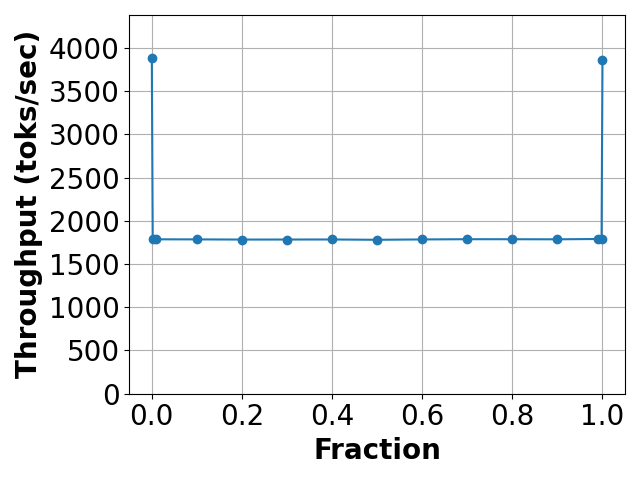
\includegraphics[width=\linewidth]{results/throughput_vs_fraction_two_fam_llama8b.png}
    \caption{Throughput vs Fraction of $A$ prefix requests}
    \label{fig:two_fam_tp}
\end{minipage}
\hfill
\begin{minipage}{0.48\columnwidth}
    \centering
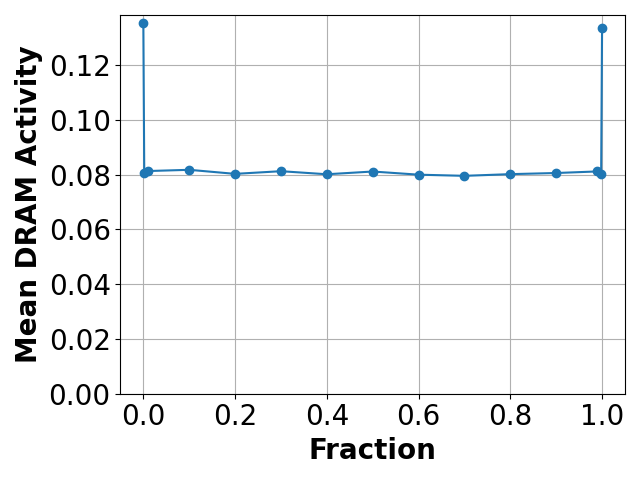
\includegraphics[width=\linewidth]{results/mean_dram_activity_vs_fraction_two_fam_llama8b.png}
\caption{Mean DRAM Activity vs Fraction of $A$ prefix requests}
\label{fig:two_fam_mean_dram}
\end{minipage}
\end{figure}




\begin{figure}[H]
\centering
\begin{minipage}{0.48\columnwidth}
    \centering
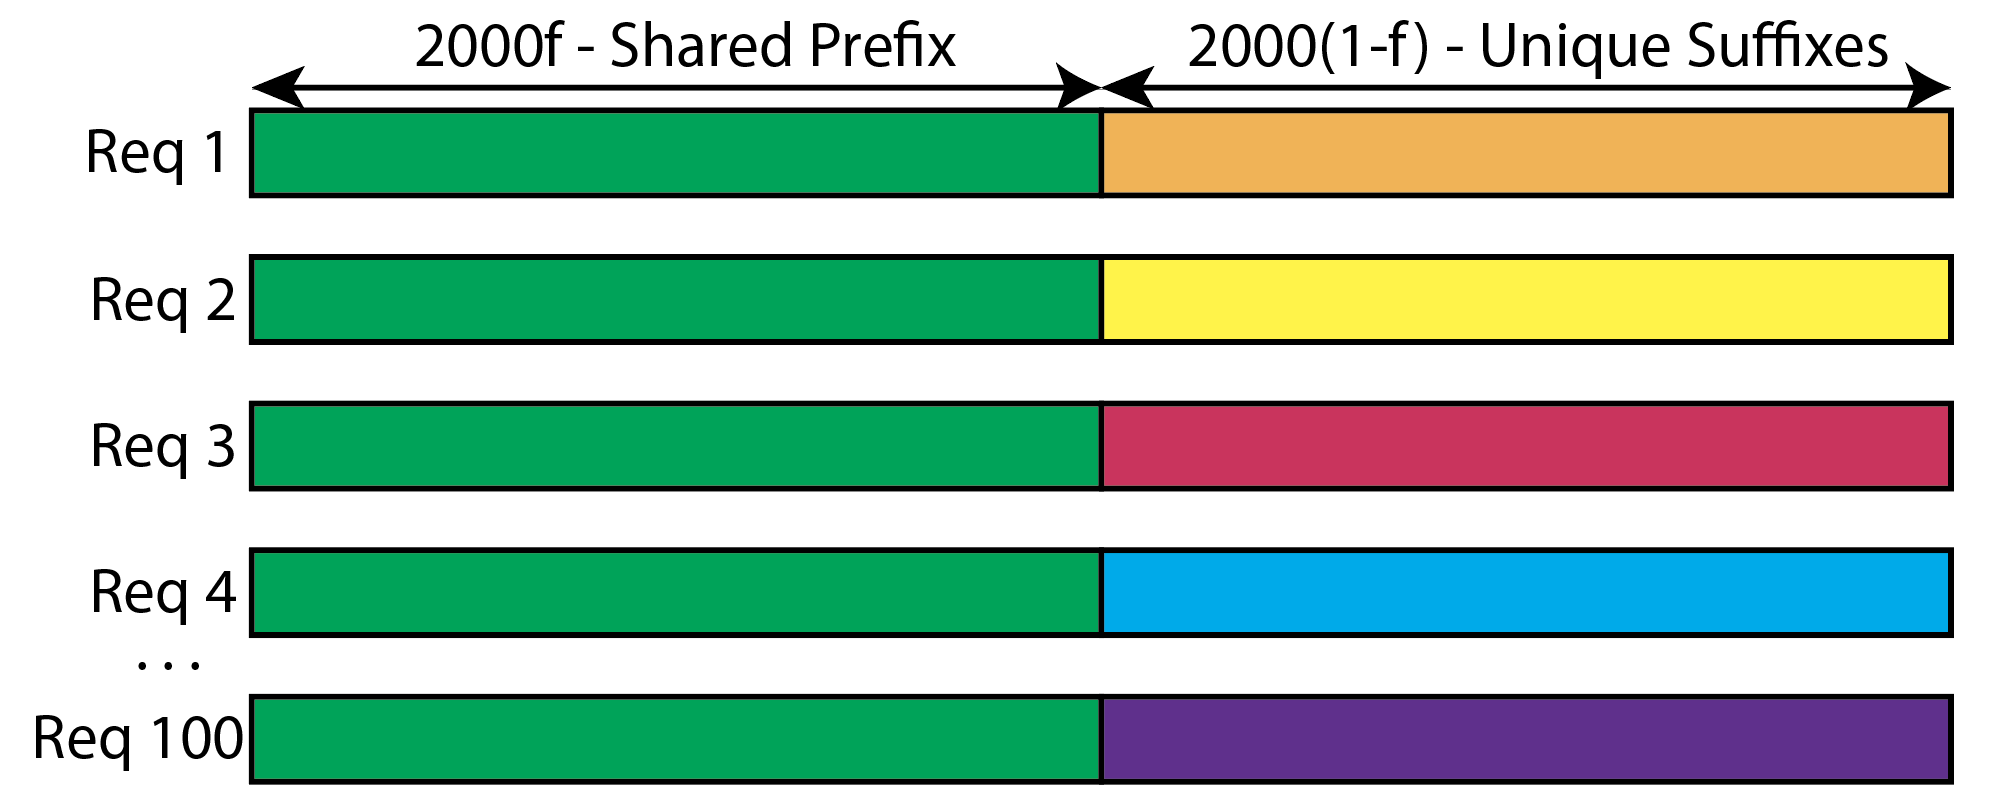
\includegraphics[width=\columnwidth]{illustration_images/fraction_sharing_experiment.png}
\caption{Visualization of $2000\times f$ tokens shared by requests}
\label{fig:frac_share_vis}
\end{minipage}
\hfill
\begin{minipage}{0.48\columnwidth}
    \centering
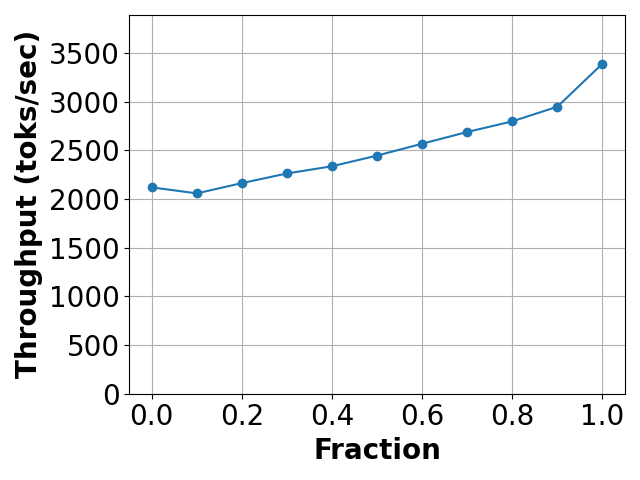
\includegraphics[width=\columnwidth]{results/throughput_vs_fraction_frac_share_llama8b.png}
\caption{Throughput vs Fraction of Sharing}
\label{fig:frac_share_tp}
\end{minipage}
\end{figure}


As shown in  Figure~\ref{fig:frac_share_tp}, there is a smooth increase in throughput with $f$. When there is no shared prefix ($f = 0$), throughput is at its lowest. As sharing increases, throughput improves consistently. When all requests share the entire prefix ($f = 1$), throughput is more than 60\% higher than in the no-sharing case. As $f$ increases, a larger portion of the KV cache becomes common across the batch. Since decode for each token repeatedly sweeps the entire KV cache, the shared region is accessed by multiple requests within a short time window, improving contiguity across memory accesses. Both temporal and spatial locality, therefore, improve with $f$, resulting in improved throughput.

\textbf{Takeaway 2:} Decode throughput increases smoothly with the amount of shared prefix across requests. Greater sharing enlarges the KV regions accessed jointly by the batch, strengthening cache reuse and improving effective memory bandwidth utilization.

The previous experiment varies only the \emph{amount} of sharing while assuming that the shared tokens appear at the beginning of the sequence. This raises a natural question: \emph{does the position of sharing within a sequence also affect decode throughput?} Our hypothesis is that because decode proceeds token by token and all requests traverse their prefixes at the same time, sharing that occurs earlier in the sequence should have a larger impact on locality than sharing that occurs later. Early shared segments allow the batch to access the same KV regions simultaneously, while later divergence breaks this alignment. To test this hypothesis, we design five sharing patterns: complete sharing, no sharing, and sharing with 2, 3, or 4 levels, as illustrated in Figure~\ref{fig:sharing_configurations}. In all configurations, the total sequence length of each request is fixed at $4L$, and only the branching structure differs. We measure decode throughput across these five settings for three values of $L$, as shown in Figure~\ref{fig:tp_vs_l_1_9_11}.

The complete sharing pattern consistently achieves substantially higher throughput than all others. This behavior is expected: full sharing preserves synchronized traversal of the KV cache throughout the entire sequence, maximizing both temporal and spatial locality.

A more subtle observation is that configurations with 2, 3, and 4 levels exhibit similar throughput across different values of $L$, despite differing branching patterns. This can be explained by the timing of memory accesses during decode. Requests within a batch issue memory accesses roughly simultaneously. During the initial shared segment of length $L$, all configurations behave identically; every request accesses the same KV region, fully exploiting locality. Once branching occurs, the batch becomes heterogeneous, and locality degrades. However, as we will show next, throughput is highly sensitive to the presence of heterogeneity but comparatively less sensitive to the exact number of distinct prefix groups once heterogeneity is introduced.  Whether the batch ultimately splits into two, four, or eight groups in later segments has only a limited additional impact since synchronized reuse has already been disrupted. Moreover, as expected, no sharing pattern achieves the lowest throughput of all.

\textbf{Takeaway 4:} Because decode-phase memory accesses from all sequences occur roughly together, the amount of sharing at the beginning of the sequence is the primary determinant of locality and throughput.



\begin{figure}[H]
    \centering
    \captionsetup[subfigure]{labelformat=simple}
    \renewcommand\thesubfigure{(\alph{subfigure})}
    \begin{subfigure}{0.25\columnwidth}
        \centering
        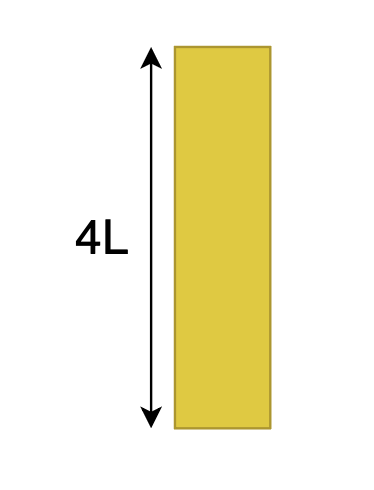
\includegraphics[width=\linewidth]{illustration_images/vis_complete_sharing.png}
        \caption{Complete sharing}
        \label{fig:vis_complete_sharing}
    \end{subfigure}
    \hfill
    \begin{subfigure}{0.35\columnwidth}
        \centering
        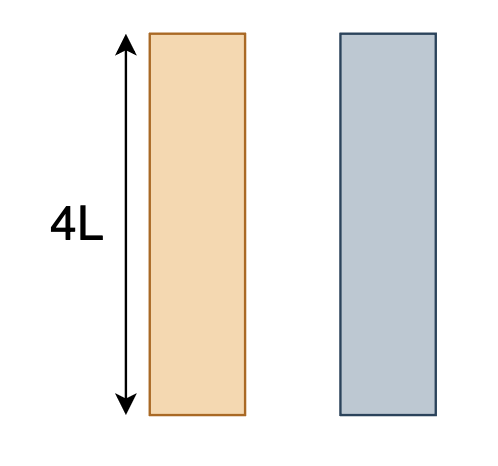
\includegraphics[width=\linewidth]{illustration_images/vis_no_sharing.png}
        \caption{No sharing}
        \label{fig:vis_no_sharing}
    \end{subfigure}
    \hfill
    \begin{subfigure}{0.35\columnwidth}
        \centering
        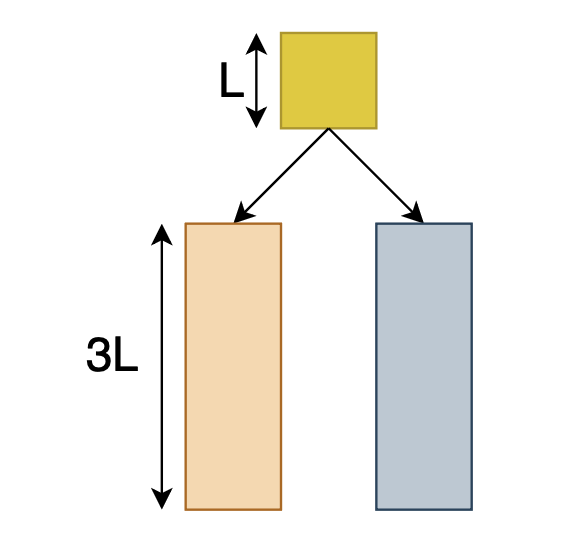
\includegraphics[width=\linewidth]{illustration_images/vis_2_levels.png}
        \caption{2 Levels}
        \label{fig:2_levels}
    \end{subfigure}

    \vspace{0.5cm}

    \begin{subfigure}{0.40\columnwidth}
        \centering
        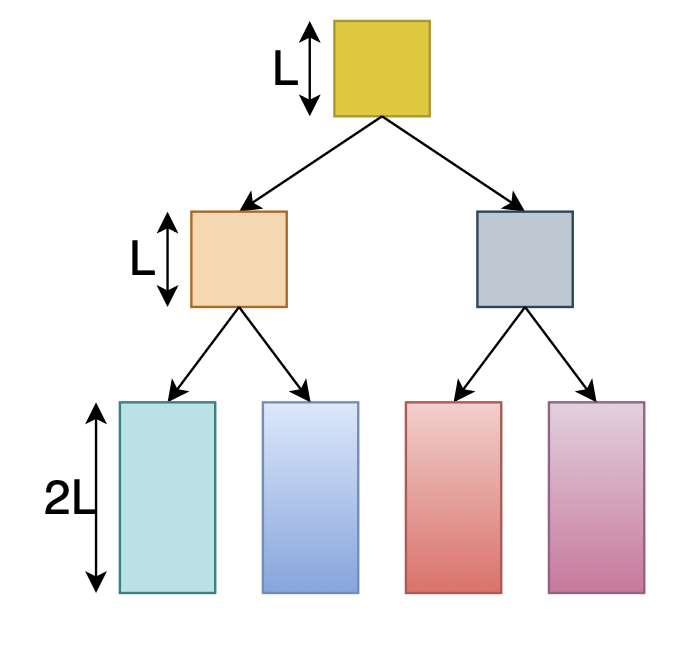
\includegraphics[width=\linewidth]{illustration_images/vis_3_levels.png}
        \caption{3 Levels}
        \label{fig:3_levels}
    \end{subfigure}
    \hfill
    \begin{subfigure}{0.58\columnwidth}
        \centering
        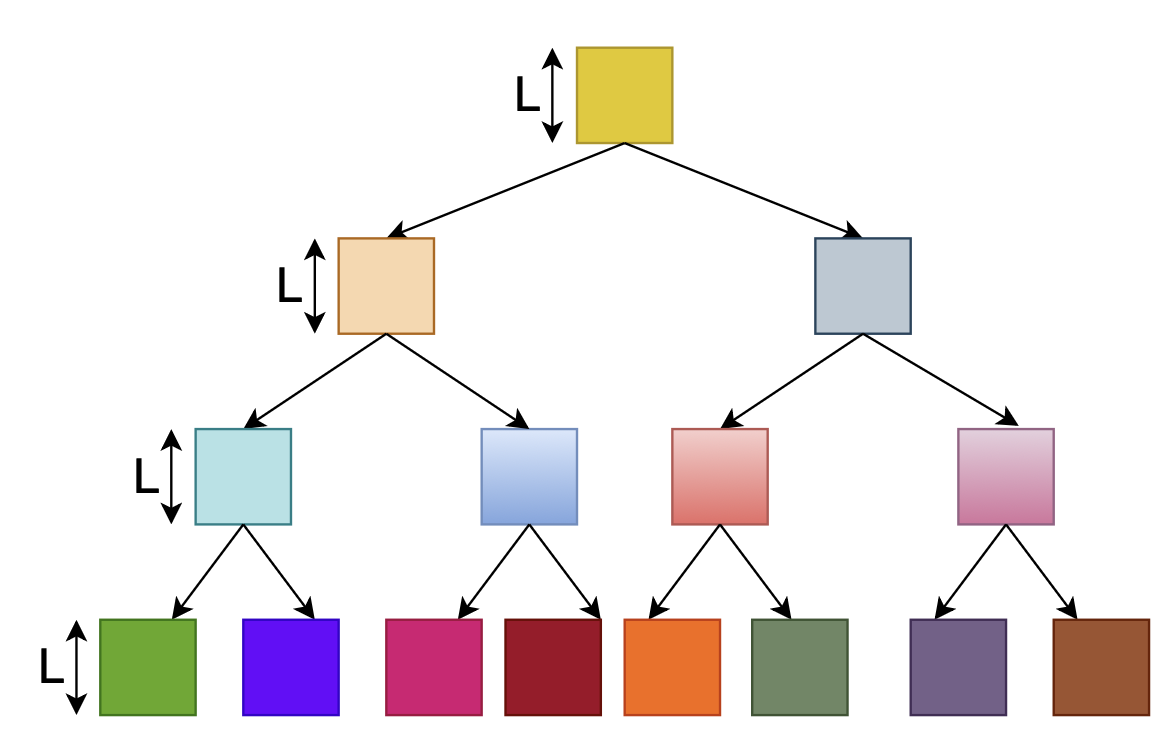
\includegraphics[width=\linewidth]{illustration_images/vis_4_levels.png}
        \caption{4 Levels}
        \label{fig:4_levels}
    \end{subfigure}

    \caption{Visualization for different sharing patterns}
    \label{fig:sharing_configurations}
\end{figure}


\begin{figure}[H]
\centering
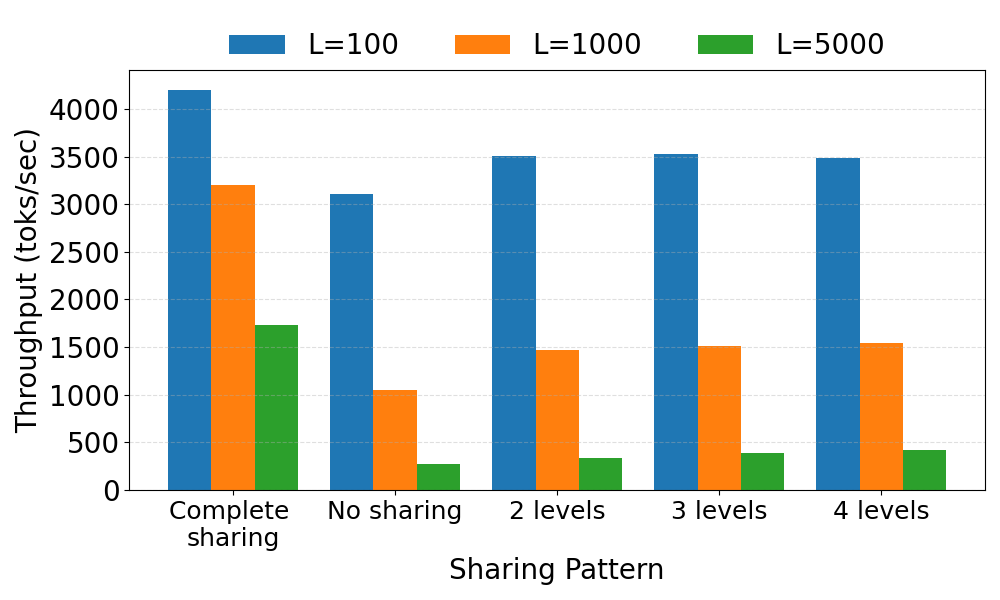
\includegraphics[width=\columnwidth]{results/tp_different_modes_sharing_at_top.png}
\caption{Throughput vs sharing patterns for different sequence lengths}
\label{fig:tp_vs_l_1_9_11}
\end{figure}

The previous experiments examine how prefix sharing affects decode throughput when the KV caches of all active requests fit within GPU memory. However, in some practical serving workloads, a system may need to handle many distinct prefixes simultaneously. This raises another important question: \emph{what happens when the number of distinct prefixes becomes large enough that their KV caches cannot all reside in GPU memory?} Our hypothesis is that when the number of active prefixes grows beyond the available GPU memory capacity, the system will be forced to evict KV cache blocks. These evictions require recomputation when the corresponding requests resume their decode phases, leading to reduced throughput and smaller effective batch sizes.

To study this effect, we construct an experiment with $N$ different shared prefixes $P_1, P_2 \dots P_N$, each of length $5000$ tokens. We create batches such that an equal number of requests corresponds to each prefix. Figure~\ref{fig:hbm_evic_tp_bs} shows the resulting throughput and average batch size as $N$ increases. As observed earlier, throughput drops when moving from $N = 1$ to $N = 2$, primarily due to reduced temporal and spatial locality. From $N = 2$ to $N = 20$, throughput remains relatively stable, indicating that locality degradation alone does not worsen performance beyond the initial heterogeneity. However, there is a sharp decline in throughput from $N = 20$ to $N = 50$. This drop occurs because the available GPU memory is no longer sufficient to hold the KV caches for all active prefixes simultaneously. This leads to frequent KV cache evictions and recomputations. The effect is also reflected in the reduced average batch size for $N = 50$ and $N = 100$, as the system cannot admit new requests due to limited GPU memory capacity. This phenomenon has also been explored in prior work~\cite{zheng2025batchllmoptimizinglargebatched,pang2025optimizingllminferencethroughput}, which highlights the impact of KV cache capacity constraints on inference throughput.

\textbf{Takeaway 4:} Beyond cache locality, the number of simultaneously active prefixes also affects performance through GPU memory capacity limits. Prefix-aware scheduling can mitigate KV cache evictions and improve throughput.

\begin{figure}[H]
\centering
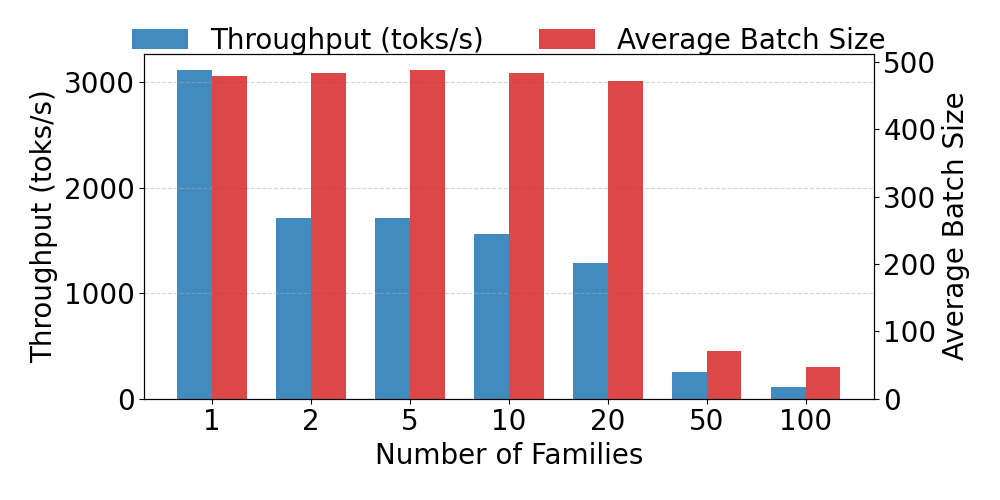
\includegraphics[width=\columnwidth]{results/hbm_evictions_fcfs_throughput_vs_batchsize_dual_axis.png}
\caption{Throughput and Average Batch Size vs Number of Prefix Groups}
\label{fig:hbm_evic_tp_bs}
\end{figure}


\subsection{Effect of Batch Size on Decode Throughput}
The previous experiments show that decode throughput is strongly influenced by prefix structure, which determines how effectively requests can reuse KV cache data. However, prefix sharing is only one factor that affects performance. Another important parameter in LLM serving systems is the \emph{batch size}, which determines how much parallel work is issued to the GPU during each decode step.

Our hypothesis is that increasing batch size should initially improve throughput by better utilizing GPU compute units, particularly tensor cores. However, once compute resources are saturated, decode performance should become limited by memory bandwidth, since each additional request increases KV cache traffic.

To study this effect, we evaluate decode phase throughput as a function of batch size. In this experiment, all the requests start from one of the 5 large prefixes of length $2000$ tokens each.  As shown in Figure~\ref{fig:batch_size_tp_motivation}, throughput increases with batch size due to improved tensor core utilization (Figure~\ref{fig:batch_size_tenso}). However, another point worth noting is that beyond a certain batch size, once the GPU’s compute units are already highly utilized, the throughput curve largely flattens. The mean SM Occupancy is shown in Figure~\ref{fig:batch_size_smocc} (\textcolor{red}{currently linked to appendix plot, can remove this}).

\textbf{Takeaway 5:} We should aim to increase the batch size to better utilize GPU compute, but only up to the point when the tensor core utilization saturates, after which decode performance is no longer limited by arithmetic throughput but by KV cache movement between HBM and on-chip caches. At that stage, simply adding more requests to the batch does not yield proportional gains because memory becomes the bottleneck.

\begin{figure}[H]
\centering
\begin{minipage}{0.48\columnwidth}
\centering
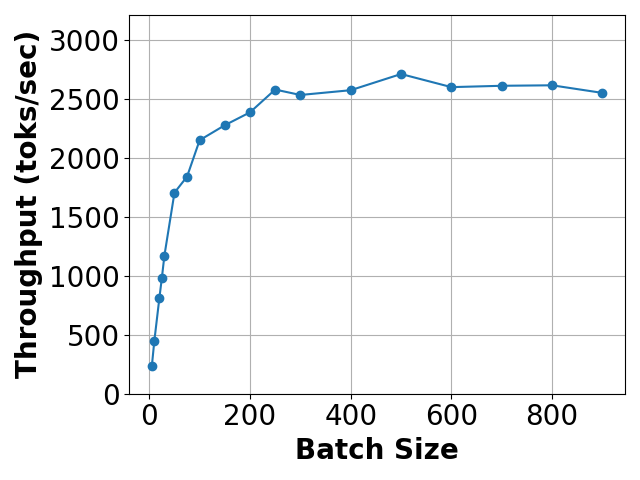
\includegraphics[width=\columnwidth]{results/throughput_vs_batch_size_llama8b.png}
\caption{Throughput vs Batch Size}
\label{fig:batch_size_tp_motivation}
\end{minipage}
\hfill
\begin{minipage}{0.48\columnwidth}
\centering
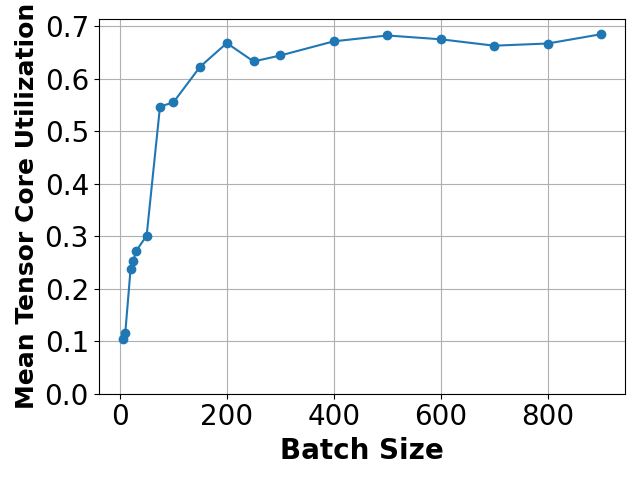
\includegraphics[width=\columnwidth]{results/mean_tenso_vs_batch_size_llama8b.png}
\caption{Tensor Core Utilization vs Batch Size}
\label{fig:batch_size_tenso}
\end{minipage}
\end{figure}


The previous experiment examined how batch size affects decode throughput under a fixed prefix structure. In practice, however, LLM serving workloads involve both \emph{prefill} and \emph{decode} phases. These two stages stress different system resources: prefill is primarily compute-intensive, while decode is largely memory-bound due to repeated traversal of the KV cache. Consequently, the benefits of prefix locality observed in earlier experiments may manifest differently when considering end-to-end execution.

Our first hypothesis is that the benefits of prefix locality should become increasingly pronounced as the decode length grows. Prefill is largely a write-heavy workload that constructs the KV cache once, while decode repeatedly reads the entire prefix at every generation step. As the number of decode tokens increases, these repeated KV sweeps amplify the impact of memory locality.

Moreover, there exists a trade-off between large heterogeneous batches and smaller prefix-homogeneous batches. Large heterogeneous batches maximize tensor core utilization, while homogeneous batches preserve aligned traversal of the KV cache during decode.

To evaluate these hypotheses, we measure end-to-end throughput, including both prefill and decode phases. Unlike previous decode-only experiments, we do not perform a warmup run; thus, prefix computation and KV cache construction are included in the reported throughput. We consider a workload consisting of eight distinct prefix groups, each containing 100 requests (800 total). We evaluate several batching strategies: (i) a single heterogeneous batch of 800 requests spanning all eight families; (ii) two batches of 400 requests covering four families each; (iii) four batches of 200 requests covering two families each; (iv) eight batches of 100 requests, each homogeneous; (v) sixteen batches of 50 requests, each homogeneous; and (vi) thirty-two batches of 25 requests, each homogeneous. We further vary the number of decode tokens to study how the prefill–decode balance influences performance.

Figure~\ref{fig:prefill_decode_tp_batch_config_decode} shows throughput across these configurations. When the decode length is small, throughput is largely influenced by prefill computation. In this regime, larger heterogeneous batches tend to perform well because they maximize tensor core utilization and arithmetic intensity during the prefix processing stage. As we progressively split the large 1×800 batch into 2×400 and 4×200 configurations, throughput decreases slightly, reflecting reduced compute efficiency from smaller batch sizes. In this setting, the benefits of memory locality are not yet dominant enough to compensate for the loss in arithmetic utilization.

However, as we increase the number of decode tokens, there is a shift in the performance trend. Decode requires each request to repeatedly sweep its entire KV cache. When batches are heterogeneous, these sweeps interleave across disjoint memory regions, weakening spatial and temporal locality. As a result, memory accesses become fragmented and effective bandwidth utilization decreases. In contrast, once we transition to fully homogeneous batches (8$\times$100), throughput increases significantly, even though each batch is smaller than the earlier configurations. This improvement arises because all requests within a batch now share the same prefix, restoring synchronized traversal of the KV cache and strengthening both spatial and temporal locality.

Interestingly, even the 16$\times$50 configuration, which further reduces batch size but remains homogeneous, continues to outperform the single large heterogeneous batch (1$\times$800) when the decode length is sufficiently large. This demonstrates that the locality benefits from prefix alignment can outweigh the loss in tensor core utilization. Only when batches become too small (32$\times$25) does throughput begin to decline again. At that point, reduced arithmetic intensity and lower tensor core occupancy dominate, and the compute under-utilization can no longer be compensated by improved memory alignment.

The impact of decode length further illustrates this trade-off. When the number of decode tokens is small (e.g., 10 tokens), a homogeneous batch of size $50$ does not outperform a heterogeneous batch of size 800, since the workload remains largely dominated by prefill computation and compute efficiency plays a larger role. However, when we increase the decode length to 100 tokens, the homogeneous 50-request batch begins to surpass the large heterogeneous batch. This occurs because each additional decode step requires another full sweep of the KV cache, allowing the benefits of aligned memory access patterns to accumulate over time. As decode length increases, execution becomes increasingly memory-bound, and the advantage of prefix-homogeneous batching becomes more pronounced.

Overall, these results highlight a fundamental balance between compute utilization and memory locality. Large heterogeneous batches maximize tensor core usage but fragment KV access patterns. Moderately sized homogeneous batches preserve aligned traversal of the KV cache and can achieve higher effective throughput when decode dominates execution. The optimal operating point lies where compute resources remain well utilized while memory access patterns remain synchronized across requests.

\textbf{Takeaway 6:} Under end-to-end execution, it is often beneficial to process requests in prefix-homogeneous batches, even if this slightly reduces batch size. As the number of decode tokens increases, repeated KV cache sweeps amplify the benefits of memory locality, allowing moderately sized homogeneous batches to outperform larger heterogeneous batches. However, this benefit holds only up to a point: when batches become too small, reduced tensor core utilization and lower arithmetic intensity lead to underutilized compute, causing throughput to decline.
\begin{figure}[H]
\centering
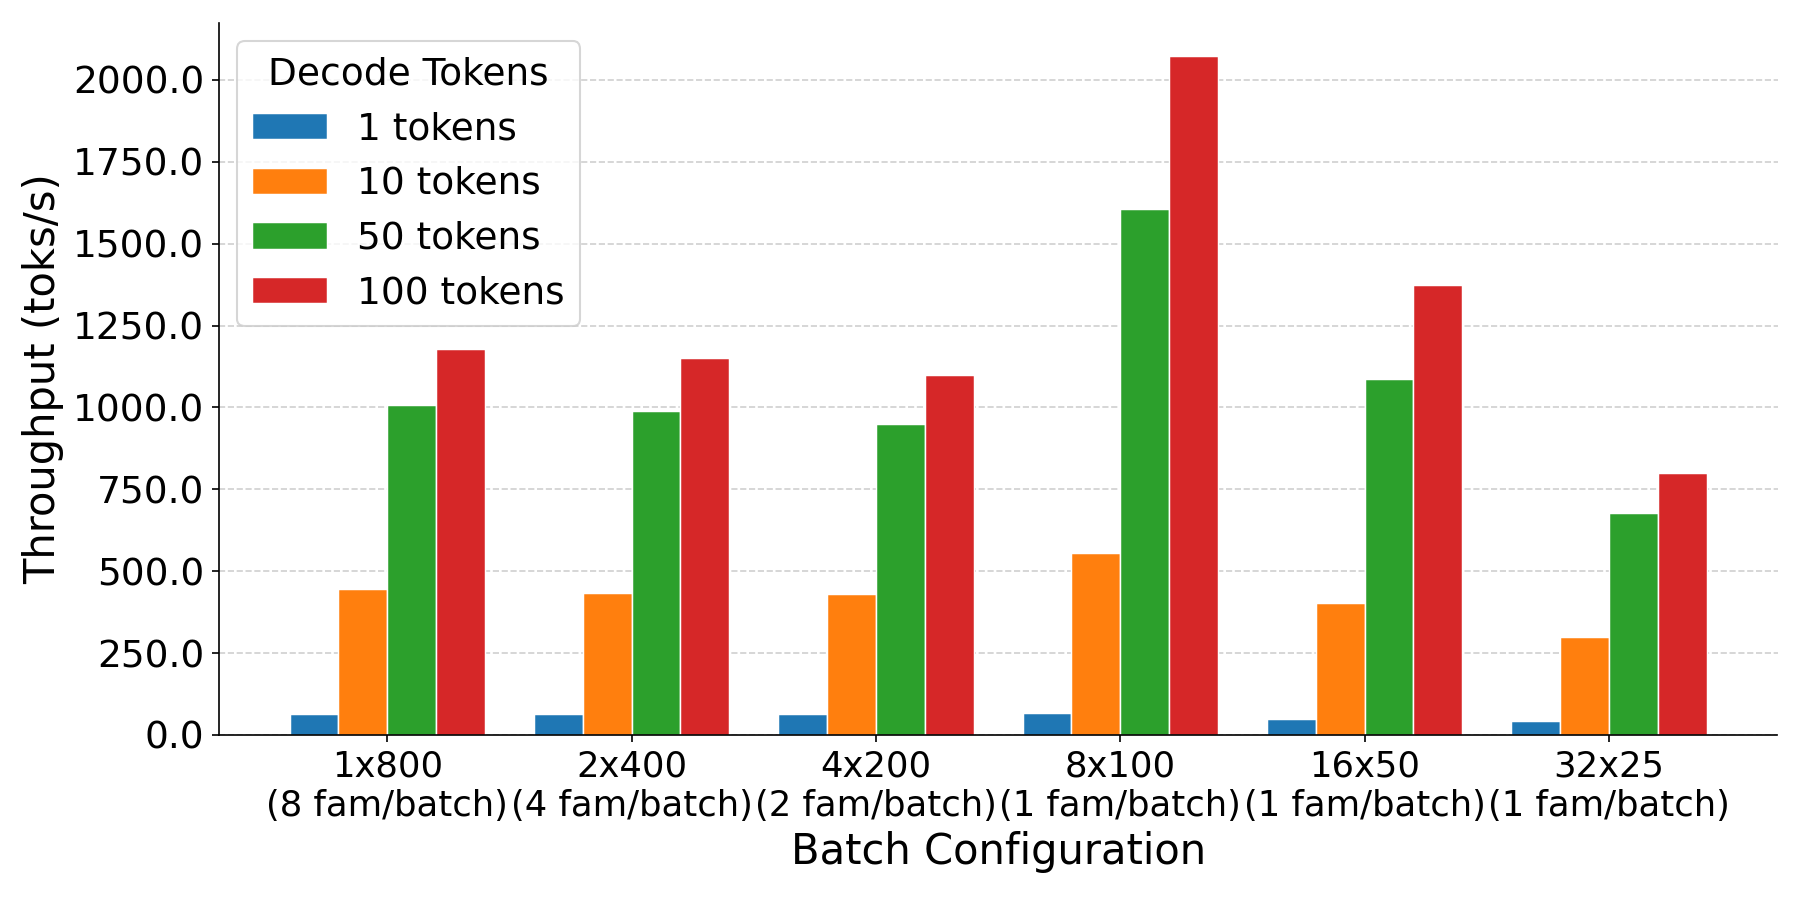
\includegraphics[width=\columnwidth]{results/prefill_decode_homo_hetero_grouped_throughput.png}
\caption{Throughput vs Batch Configurations for varying number of decode tokens}
\label{fig:prefill_decode_tp_batch_config_decode}
\end{figure}


\subsection{Overhead of dynamic prefix detection}
So far, we have analyzed how the prefix sharing structure and batch size affect the overall inference throughput. Next, we plan to study how the state-of-the-art inference engines identify prefix sharing and what the overall cost involved in doing this is. Although existing inference engines such as SGLang \cite{zheng2024sglangefficientexecutionstructured} and BatchLLM \cite{zheng2025batchllmoptimizinglargebatched} do not consider making the batch prefix-homogeneous, they still attempt to detect prefix sharing using radix trees to schedule requests in an order that minimizes KV cache recomputations. In SGLang, two radix-tree-aware scheduling policies are proposed. The first, \emph{Longest Prefix Match (LPM)}, prioritizes requests whose input prefixes match the longest cached prefixes \textcolor{red}{a better definition needed here?}. The second, \emph{DFS-Weight}, performs a depth-first traversal of the radix tree and prioritizes branches that have more active requests. To understand the overhead of these scheduling policies, we implemented a radix-tree-based scheduler inside vLLM and measured its CPU cost. We constructed a workload of 2000 requests, each with a 10k-token prefix, and compared the CPU time spent on scheduling against the total execution time. We also compared these results with an idealized policy in which the user directly provides prefix group identifiers, eliminating the need for any dynamic prefix discovery. \textcolor{red}{describe prefix aware attention here, after reading through, and check if it matches on what we have implemented}

Table~\ref{tab:cost_schedulers} shows the results. SGLang’s LPM and DFS-Weight policies incur 78.24 and 89.06 seconds of CPU time, respectively, on the same order as the GPU computation. Our radix-tree implementation in vLLM reduces this overhead somewhat (57.53 seconds), but the cost remains substantial. In contrast, when prefix group identifiers are provided explicitly, the CPU overhead drops to just 0.03 seconds.

There is a structural reason for this gap: radix trees require token-by-token comparisons during insertion, dynamic node splitting when partial matches occur, and the maintenance of shared paths as requests arrive and complete. Scheduling decisions further require repeated traversals of the tree. With long prompts and high concurrency, these operations accumulate significant constant-factor overhead. 

\textbf{Takeaway 7:} Existing approaches introduce significant CPU overhead while detecting prefix sharing, which is at times even comparable to the GPU execution time. 
\begin{table}[t]
\centering
\small
\resizebox{\columnwidth}{!}{\begin{tabular}{lcccc}
\toprule
\textbf{Policy} & \textbf{Batch Time (s)} & \textbf{Exec (s)} & \textbf{Throughput} & \textbf{TC Util.} \\
\midrule
vLLM FCFS & 3e-6 & 229.36 & 436.25 & 0.67 \\
vLLM User IDs & 0.03 & 105.43 & 948.54 & 0.336 \\
vLLM RadixTree & 62.95 & 139.33 & 717.35 & 0.20 \\
SGLANG DFS-W & 92.15 & 177.78 & 562.61 & 0.22 \\
SGLANG LPM & 46.62 & 149.27 & 669.92 & 0.26 \\
\bottomrule
\end{tabular}}
\caption{Comparison of scheduling policies}
\label{tab:cost_schedulers}
\end{table}

\textcolor{red}{add prefix aware attention tree after reading the paper and implementing their idea}

\textcolor{red}{remove vllm radix tree as it has our own optimizations, or we can keep it still?}

\textcolor{red}{batchLLM avoids this cost by shifting to offline serving, similar to blendserve.}


